\documentclass[11pt, letterpaper]{article}
\usepackage[utf8]{inputenc}
\usepackage{graphicx}
\graphicspath{{images/}}
\usepackage{amsmath}
\usepackage{amssymb}
\usepackage{fancyhdr}

\pagestyle{fancy}
\fancyhf{}
\rhead{ECE 316 Chapter 2}
\lhead{Spring 2017}
\rfoot{\thepage}
\title{ECE316 Lecture Note 2 by Prof. Xie - Spring 2017}
\author{Prof. Liang-Liang Xie}
\date{\today}
\begin{document}
\setcounter{section}{1}
\section{Axioms of Probability}
\subsection{Introduction}
\subsection{Sample Space and Events}
$\mathit{S}$ - Sample space: the set of all possible outcomes of an experiment. \\
\begin{enumerate}
  \item Flip a coin, $S = \{ \text{tail,  head} \}$
  \item Flip two coins, $S = \{(H,H), (T,T), (H,T), (T,H)\}$.
  \item Toss two dices, $S = \{(i,j): i,j=1,2,3,4,5,6\}$
  \item The order of finish in a race among 7 horses. \\ $S = \{ \text{all } 7! \text{ permutations of } (1,2,3,4,5,6,7) \}$
  \item Measuring (in hours) the life time of a transistor. \\ $S = \{x:0 \le x < +\infty \}$
\end{enumerate}
\vspace{1.0cm}
\textit{Event} - Any subset of $E$ of the sample sapce is known as an event. \\ That is, an event is a set of some possible outcomes. \\ If the outcome of the experiment is contained in $E$, then we say the $E$ has occurred.
\begin{enumerate}
  \item $E = \{\text{head}\}, F = \{\text{tail}\}$
  \item $E = \{(H,H), (H,T)\}$ - The first coin is head. \\ $F = \{(T,H), (H,T)\}$ - The two coins have different appearances.
\end{enumerate}
For $E$, obviously, if $(H,H)$ happens, we can say it happens that the first coin is head. This explains that if the outcome of the experiment is contained in $E$, then we say the $E$ has occurred.
\begin{enumerate}
  \setcounter{enumi}{2}
  \item $E = \{(1,6), (2,5), (3,4), (4,3), (5,2), (6,1)\}$ - The sum of the dice is 7.
  \item $E = \{\text{all permutations starting with 3}\}$ - Horse 3 wins the race.
  \item $E = \{x:0 \le x \le 5\}$ - The transistor last longer than 5 hours.
\end{enumerate}
\clearpage
\noindent
We can define,
\begin{itemize}
  \item $E \cup F$ - the union of two events.
  \item $EF\text{ (}E \cap F\text{)}$ - the intersection of two events.
  \item $E_1 \cup E_2 \cup E_3 \dots = \bigcup_{n=1}^\infty E_n$
  \item $E_1 \cap E_2 \cap E_3 \dots = \bigcap_{n=1}^\infty E_n$
  \item What if $E_1$ and $E_2$ have no common outcomes? $E_1E_2 = \varnothing$
  \item $E^c = $\{all outcomes not in $E$\}; $S^c = \varnothing$
  \item $E \subset F$ implies that all elements in $E$ are contained by $F$. It implies that if $E$ occurs, we can say $F$ occurs.
  \item $E \subset F \Leftrightarrow F \supset F$
  \item If $E \subset F$ and $F \subset E$, then $E=F$
\end{itemize}
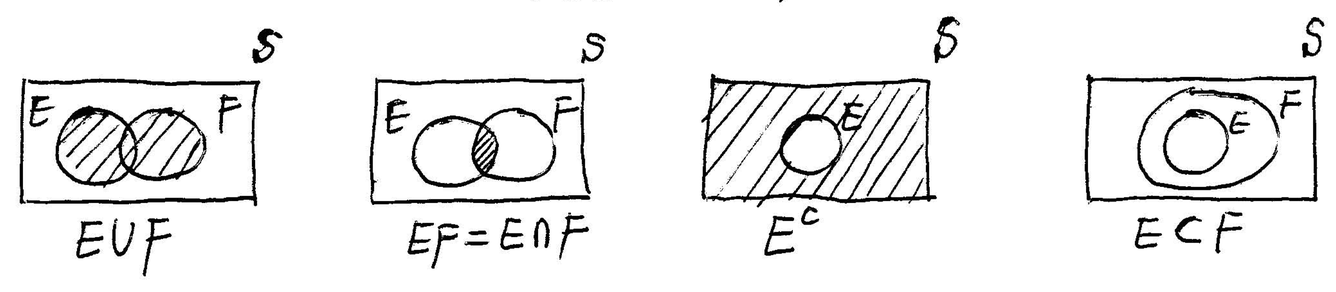
\includegraphics[scale=0.5]{2-1} \\
\begin{tabular}{l l}
  Commutative laws & $E \cup F = F \cup E$, \quad $EF = FE$ \\
  Associative laws & $(E \cup F) \cup G = E \cup (F \cup G)$, \quad $(EF)G = E(FG)$ \\
  Distributive laws & $(E \cup F)G  = (EG) \cup (FG)$, \quad $(EF) \cup G = (E \cup G)(F \cup G)$
\end{tabular} \\ \\
\noindent
\textit{Proof of Distributive laws:} \\
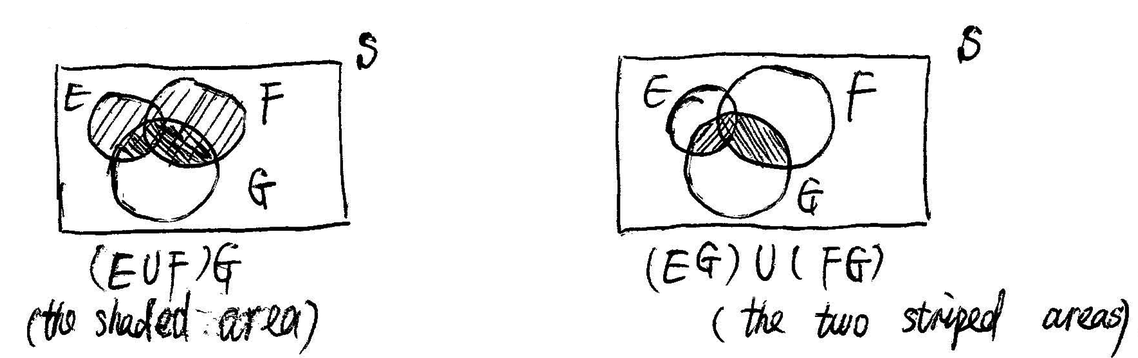
\includegraphics[scale=0.3]{2-2}
\clearpage
\textit{Similarly,} \\
\begin{center}
  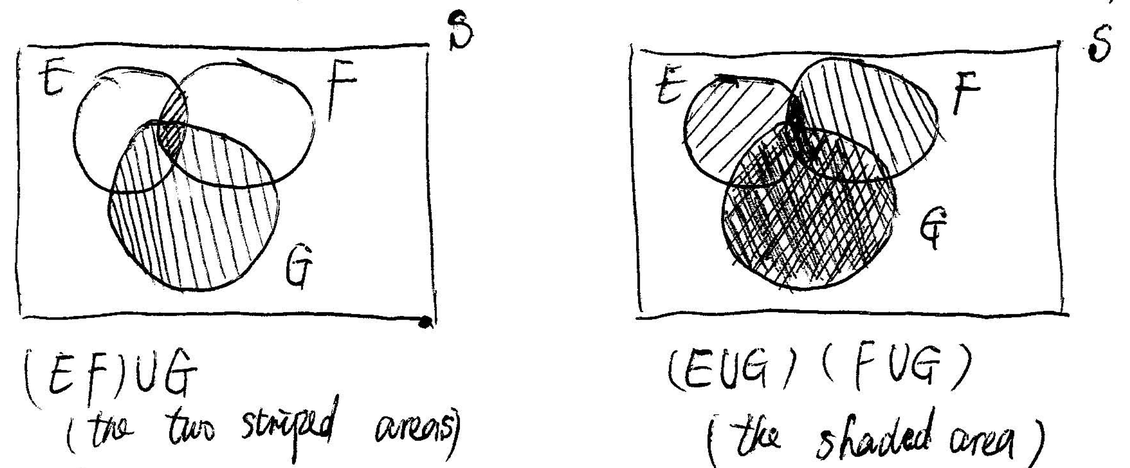
\includegraphics[scale=0.55]{2-3}
\end{center}
DeMorgan's Law \\
\begin{align*}
  \left(\bigcup_{i=1}^n E_i\right)^c &= \bigcap_{i=1}^n {E_i}^c \\
  \left(\bigcap_{i=1}^n E_i\right)^c &= \bigcup_{i=1}^n {E_i}^c
\end{align*}
\begin{tabular}{l l}
  \textit{Proof:} & Suppose $x \in \left(\bigcup_{i=1}^n E_i\right)^c$ \\
                  & then, $x \not\in \bigcup_{i=1}^n E_i$, \\
                  & then, $x \not\in E_i$, for any(all) $i = 1,2,3\dots,n$. \\
                  & then, $x \in {E_i}^c$, for any(all) $i = 1,2,3\dots,n$. \\
                  & then, $x \in \bigcap_{i=1}^n {E_i}^c$
\end{tabular}
\begin{equation*}
  \therefore \left(\bigcup_{i=1}^n E_i \right)^c \subset \bigcap_{i=1}^n {E_i}^c
\end{equation*} \\
Similarly, we can get $\bigcap_{i=1}^n {E_i}^c \subset \left(\bigcup_{i=1}^n E_i \right)^c$ \\
$\therefore$ the two sets are contained by each other, and if $A \subset B, B \subset A$, then $A=B$. Therefore, $\left(\bigcup_{i=1}^n E_i \right)^c = \bigcap_{i=1}^n {E_i}^c$
\clearpage
\subsection{Axioms of Probability}
$S$ - sample space, $E$ - Event \\ \\
\begin{tabular}{l l}
  Axiom 1 & $0 \le P(E) \le 1$, for any event $E$. \\
  Axiom 2 & $P(S) = 1$ \\
  Axiom 3 & For any sequence of mutually exlusive events $E_1,E_2\dots$ \\
          & (that is, $E_iE_j=\varnothing$, when $i \not= j$) \\
          & $P\left(\bigcup_{i=1}^\infty E_i \right) = \sum_{i=1}^\infty P(E_i)$
\end{tabular} \\ \\
\noindent
\textbf{Example}: Measuring (in hours) the lifetime of a transistor
\begin{align*}
  S &= \{ x: 0 \le x \le \infty \} \\
  \text{let } E_i &= \{ x_i: i-1 \le x < i \}, i=1,2,3 \dots
\end{align*}
\begin{center}
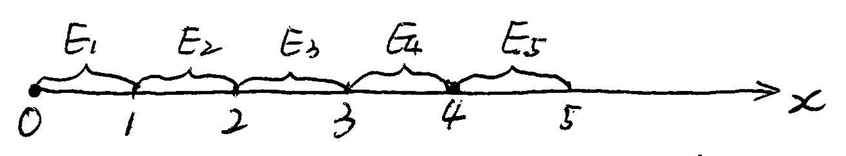
\includegraphics[scale=0.5]{2-4}
\end{center}
\begin{equation*}
  P(E_1) = \frac{1}{2}, \quad P(E_2) = \frac{1}{4}, \quad P(E_3) = \frac{1}{8} \dots P(E_i) = \frac{1}{2^i}
\end{equation*} \\
\begin{align*}
  P \left( \bigcup_{i=1}^\infty E_i\right) &= P(S) = 1 \\
  \sum_{i=1}^\infty P(E_i) &= \sum_{i=1}^\infty \frac{1}{2^i} = \frac{1}{2} + \frac{1}{4} + \frac{1}{8} + \dots = 1 \\
  \therefore \quad P \left( \bigcup_{i=1}^\infty E_i \right) &= \sum_{i=1}^\infty P(E_i), \text{ which confirms the axiom 3.} \\
  P \left( \bigcup_{i=1}^\infty E_i\right) &= \sum_{i=1}^\infty P(E_i) \Rightarrow P \left( \bigcup_{i=1}^n E_i\right) = \sum_{i=1}^n P(E_i)
\end{align*} \clearpage
Choose $E_1 = S$, $E_2 = \varnothing$, $E_3 = \varnothing$, $E_4 = \varnothing$, $\dots$ ($E_iE_j = \varnothing$, when $i \not= j$). \\
\begin{align*}
  \text{then, } P \left( \bigcup_{i=1}^\infty E_i \right) &= P(S) \\
  \sum_{i=1}^\infty P(E_i) &= P(S) + P(\varnothing) + P(\varnothing) + P(\varnothing) + \dots \\
  \text{By axiom 3, } P(S) &= P(S) + P(\varnothing) + P(\varnothing) + P(\varnothing) + \dots \\
  \therefore P(\varnothing) &= 0
\end{align*} \\
To prove $\left( \bigcup_{i=1}^n E_i\right) = \sum_{i=1}^n P(E_i)$ \\
\begin{align*}
  &\text{let } E_{n+1} = \varnothing, E_{n+2} = \varnothing, \dots \\
  &\text{then, } \bigcup_{i=1}^\infty E_i = \bigcup_{i=1}^n E_i, \quad P(E_{n+1}) = 0, \quad P(E_{n+2}) = 0, \dots \\
  \therefore \quad &P \left( \bigcup_{i=1}^\infty E_i \right) = \sum_{i=1}^\infty P(E_i) \text{ implies } P \left( \bigcup_{i=1}^\infty E_i \right) = \sum_{i=1}^n P(E_i)
\end{align*} \\ \\
\noindent
\textbf{Example}: Toss a coin, if a head is as likely as a tail, then
\begin{equation*}
  P(\{H\}) = P(\{T\}) = \frac{1}{2}
\end{equation*}
If the coin is biased, $P(\{H\}) = \frac{2}{3}, P(\{T\}) = \frac{1}{3}$
\textbf{Example}: Roll a die, if all sides are equally likely,
\begin{align*}
  P(\{1\}) &= P(\{2\}) = P(\{3\}) = P(\{4\}) = P(\{5\}) = P(\{6\}) = \frac{1}{6} \\
  P(\{2,4,6\}) &= P(\{2\} \cup \{4\} \cup \{6\}) = P(\{2\}) + P(\{4\}) + P(\{6\}) = 3 \times \frac{1}{6} = \frac{1}{2}
\end{align*} \clearpage
\subsection{Some Simple Propositions}
\textit{Proposition 4.1.} $P(E^c) = 1 - P(E)$
\begin{align*}
   \hspace{1.2cm} \textit{\underline{Proof}: } &E^c \cup E = S, \quad E^c \cap E = \varnothing \\
   &P(S) = P(E) + P(E^c), \text{ due to } P\left(\bigcup_{i=1}^n E_i \right) = \sum_{i=1}^n P(E_i) \\
  &\therefore \quad P(E) + P(E^c) = 1, \\
  &\therefore \quad P(E^c) = 1 - P(E)
\end{align*}
\textit{Proposition 4.2. } If $E \subset F$, then $P(E) \le P(F)$
\begin{align*}
  \textit{\underline{Proof}: } &F = E \cup (E^cF) \\
  &\therefore P(F) = P(E) + P(E^cF) \\
  &\text{Since, } P(E^cF) \ge 0, \text{ } \therefore P(E) \le P(F)
\end{align*}
\textit{Proposition 4.3. } $P(E \cup F) = P(E) + P(F) - P(EF)$ \\
\textit{Proposition 4.4. }
\begin{align*}
  P(E \cup F \cup G) &= P(E) + P(E) + P(E) \\
  &- P(EF) - P(EG) - P(FG)  \\
  &+ P(EFG)
\end{align*}
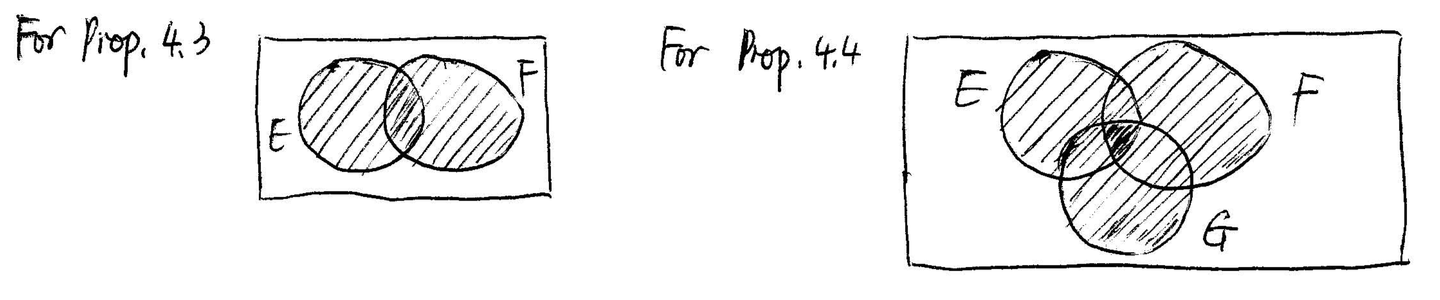
\includegraphics[scale=0.5]{2-5} \\
Think of $P(E \cup F)$ and $P(E \cup F \cup G)$ as the striped area respectively in the above two Venn diagram. By calculating the areas of the two striped regions, we can get proposition 4.3 and 4.4 respectively.
\begin{align*}
  P(E \cup F \cup G \cup H) &= P(E) + P(F) + P(G) + P(H) \\
  &- P(EF) - P(EG) - P(EH) - P(FG) - P(FH) - P(GH) \\
  &+ P(EFG) + P(EFH) P(EGH) + P(FGH) \\
  &- P(EFGH)
\end{align*} \clearpage
\noindent
\textbf{Example: } Mike is going to take two courses A and B next term. With probability 0.8, he will like course A. With probability 0.7, he will like course B. With probability 0.6, he will like both courses. What's the probabilitythat he will like neither course? \\ \\
\noindent
\underline{Solution}:
\begin{align*}
  &E = \{ \text{Mike will like course A} \}; F = \{ \text{MIke will like course B} \} \\
  &\text{then, } E \cup F = \{ \text{Mike will like at least one of them} \} \\
  &\text{Since } P(E \cup F) = P(E) + P(F) - P(EF)  = 0.8 + 0.7 -0.6 = 0.9 \\
  \therefore \quad &P\{ \text{Mike will like neither} \} = 1 - P(E \cup F) = 1 - 0.9 = 0.1
\end{align*}
\subsection{Sample space having equally likely outcomes}
\begin{align*}
  &S = \{1,2, \dots N \} \\
  &P(\{1\}) = P(\{2\}) = \dots = P(\{N\}) = \frac{1}{N} \\
  \text{Therefore, } &P(E) = \frac{\text{number of outcomes in } E}{\text{total number of outcomes in } S}
\end{align*}
\textbf{Example: } If two dice are rolled, what's the probability that the sum of the dice will equal to 7? \\ \\
\noindent
\underline{Solution}:
\begin{align*}
  E_7 &= \{\text{the sum of the dice will equal to 7}\} \\
  &= \{ (1,6), (2,5), (3,4), (4,3), (5,2), (6,1) \} \\
  &\text{The total number of outcomes in $S$ is $6\times6 = 36$.} \\
  \therefore \quad P(E_7) &= \frac{6}{36} = \frac{1}{6} \\
  &\text{Similarly, } E_6 = \{(1,5), (2,4), (3,3), (4,2), (5,1)\} \\
  \therefore \quad P(E_6) &= \frac{5}{36}
\end{align*}
\noindent
\textbf{Example: } A room of $n$ people. What's the probability that no two of them celebrate their birthday on the same day of the year? How big should $n$ be such that the probability is less than $\frac{1}{2}$? \clearpage

\noindent
\underline{Solution}: As each person can celebrate his or her birthday on any one of 365 days, there is a total of $365^n$ possible outcomes. Then the desired probability is
\begin{equation*}
  P_0 = \frac{(365)(364)(363)\dots(365-n+1)}{365^n}
\end{equation*}
Since $P_0$ is non-increasing with $n$, we can calculate the $P_0$ for the specific value of $n$ and find out when $n \ge 23$, this probability is less than $\frac{1}{2}$. That is, if there are 23 or more people in a room, then the probability that at least two of them have the same birthday exceeds $\frac{1}{2} \quad i.e. \quad (1-P_0) > \frac{1}{2}$. Furthermore, we can continue to get the following results:
\begin{align*}
  \text{when } n &= 50, \quad 1 - P_0 \approxeq 97\% \\
  \text{when } n &= 100, \quad 1 - P_0 \approxeq 1 - \frac{1}{3,000,000}
\end{align*}

% inclass example
\noindent
\textbf{Example: } $N$ men at a party throws his hat into the center of the room, and then each randomly selects a hat. What's the probability that none of the men selects his own hat?
\end{document}
